\documentclass[tikz,border=2pt]{standalone}
\usepackage{amsmath}
\usetikzlibrary{arrows.meta,decorations.pathreplacing}
\begin{document}
% Whole life annuity-due for one lifetime: unit payments at 0, 1, ..., K_x while alive, none at K_x + 1,
% so Y is an annuity certain with K_x + 1 payments: Y = sum_{k=0}^{K_x} v^k = (1 - v^{K_x+1})/d.
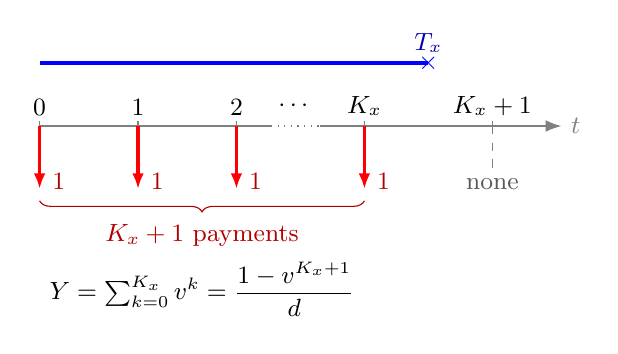
\begin{tikzpicture}[font=\small, >={Latex[length=2mm]}, x=1.25cm]
  \draw[gray] (0,0) -- (2.35,0);
  \draw[gray, dotted] (2.35,0) -- (2.85,0);
  \draw[gray, ->] (2.85,0) -- (5.3,0) node[right] {$t$};
  \foreach \t/\l in {0/0,1/1,2/2,3.3/K_x,4.6/K_x+1} {
    \draw[gray] (\t,-0.07) -- (\t,0.07);
    \node[above, inner sep=2pt] at (\t,0.05) {$\l$};
  }
  \node at (2.6,0.25) {$\cdots$};
  % the life
  \draw[blue, very thick] (0,0.8) -- (3.95,0.8);
  \node[blue] at (3.95,0.8) {$\times$};
  \node[blue!70!black, above, inner sep=2pt] at (3.95,0.85) {$T_x$};
  % payments while alive
  \foreach \t in {0,1,2,3.3} \draw[red, very thick, ->] (\t,0) -- (\t,-0.8);
  \node[red!70!black, anchor=west] at (0.03,-0.7) {$1$};
  \node[red!70!black, anchor=west] at (1.03,-0.7) {$1$};
  \node[red!70!black, anchor=west] at (2.03,-0.7) {$1$};
  \node[red!70!black, anchor=west] at (3.33,-0.7) {$1$};
  \draw[gray, dashed] (4.6,0) -- (4.6,-0.55);
  \node[gray!70!black, anchor=north] at (4.6,-0.55) {none};
  \draw[red!70!black, decorate, decoration={brace, mirror, amplitude=4pt}] (0,-0.95) -- (3.3,-0.95)
    node[midway, below=5pt] {$K_x+1$ payments};
  \node[anchor=north] at (1.65,-1.6) {$Y=\sum_{k=0}^{K_x}v^k=\dfrac{1-v^{K_x+1}}{d}$};
\end{tikzpicture}
\end{document}
